\section{Laboratory work implementation}

\subsection{Tasks and Points}

\begin{itemize}
	\item Realizeaza un site cu folosirea maximala a tagurilor
	\item Pentru formatarea paginilor se va folosi CSS
	\item Site-ul trebuie sa pastreze toata informatia intr-o baza de date
	\item Site-ul trebuie sa contina AJAX Requests.
	\item Implimentarea XHR sau JSON responses. Careva din informatie trebuie sa fie dinamic incarcata pe pagina.
\end{itemize}

\subsection{Analiza lucrarii de laborator}
Repository \href{https://github.com/AScripnic/MIDPS-laboratories/tree/master/Lab%233}{link}\par

Primul pas spre elaborarea task-urilor puse a fost setarea unui module bundler și anume webpack \cite{webpack} cu scopul de a face un proces cât mai simplu si rapid de lucru cu dependețe externe și alte facilități care le voi descrie în continuare.\par

După setare \href{https://github.com/AScripnic/MIDPS-laboratories/blob/master/Lab%233/website/webpack.config.js}{configului} de bază pentru webpack am instalat alte tooluri necesare pentru crearea unui website care sunt:

\begin{itemize}
 \item babel-loader: care permite utilizarea celor mai noi versiuni a limbajului javascript - ES6\cite{es6}
 \item sass-loader: care permite scriei css-ului intr-o metodă cât mai optimală și rezervată sass\cite{sass} și includerea lui direct in index.html file la execuție pentru consumul minimal de resurse.
\end{itemize}

La fel webpack mi-a mermis să fac un bundle proiectului meu, ce sporește viteza și consumul de resurse de către website.

Apoi am salvat ultima versie stabilă de angular\cite{angular} framework pe bază căruia am și construit toată aplicația.

Al doilea pas în crearea aplicației a fost crearea \href{https://github.com/AScripnic/MIDPS-laboratories/tree/master/Lab%233/website/app}{structurii fișierelor} pentru păstrarea directive-lor, controller-ilor, template-urilor și restu datelor.

Din start am determinat un \href{https://github.com/AScripnic/MIDPS-laboratories/blob/master/Lab%233/website/app/module/ng-routes.js}{routing} pentru aplicație și am determinat de ce pagini voi avea nevoie. Apoi am început crearea aplicației statice într-un asemenea format, pentru a putea ușor adăuga content dinamic care va fi primit din partea serverului.

Pentru partea de UI am creat urmatoarele pagini care la rândul lor sunt completate dinamic:
\begin{itemize}
	\item Home - unde este afișată lista de teme disponibile. reference:(\ref{home-page})
	\item Board (temă) - unde se afișează toate discuțiile pe o anumita temă reference:(\ref{board-page}) și are forma de adăugare a unei discuții noi reference:(\ref{new-thread})
	\item Thread (discuție) - unde se afișează toate commentariile la o discuție reference:(\ref{thread-page}) și adăugarea unui nou commentariu reference:(\ref{new-post})
\end{itemize}

Al treilea pas după ce am finisat partea statică a website-ului am început crearea serverului pe NodeJS\cite{nodejs} și ca framework de bază pentru ridicarea unui server pe dispozitiv am folosit ExpressJS\cite{expressjs} care mi-a dat posibilitatea de a crea \href{https://github.com/AScripnic/MIDPS-laboratories/blob/master/Lab%233/server/app.js#L22}{rute virtuale} pentru citirea imaginilor care vor fi pe partea serverului și un REST-API care mi-ar permite sa creez posturi și threaduri în aplicație mea.

Cel mai greu pas a fost încărcarea unei imagini cât pe partea de client cât și pe partea serverului. Pentru a încărca o imagine pe server am folosit modulu exterior multer\cite{multer} care făcea handle la asemenea cazuri, iar pentru partea client am folosit o directive populară, destinată framework-ului angular, ng-file-upload\cite{file-upload} care la rândul său făcea handle la evenimente de genul upload.

După încărcarea fiecărei imagini am folosit modulul jimp\cite{jimp}, care permite editarea unei imagini, pentru a crea un preview, căci clientul să nu fie nevoit să fac download la toate imaginile în marimea lor originală, și le stocam aparte.

Al patrulea pas a fost adăugarea unei baze de date, care ar permite lucru ușor și rapid cu o cantitate mai mică de date. Am ales lokijs\cite{lokijs} care lucrează cu fișiere de tip JSON, ce imi este cel mai convinabil.

Și ultimul pas a fost conectarea părții client cu server, care am făcut-o prin intermediul directivei angular \$http\cite{angular-http} care la rândul său face \href{https://github.com/AScripnic/MIDPS-laboratories/blob/master/Lab%233/website/app/services/threadService.js}{apeluri externe} de trimitere si primere a informatiei.

NOTĂ: Unica asemănare dintre 4chan și 3chan este design, în rest, javascript code, styles code și server-ul nu au nimic în comun, totul a fost creat de la zero. (nici html nu coincide).

\subsection{Imagini}
\begin{center}
	\begin{figure}[h]
		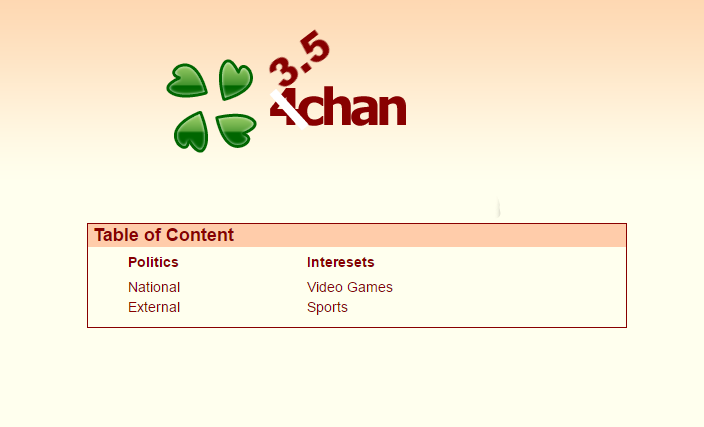
\includegraphics[scale=0.8]{home-page}\\
		\caption{Home Page}
		\label{home-page}
	\end{figure}
	
	
	\begin{figure}[h]
		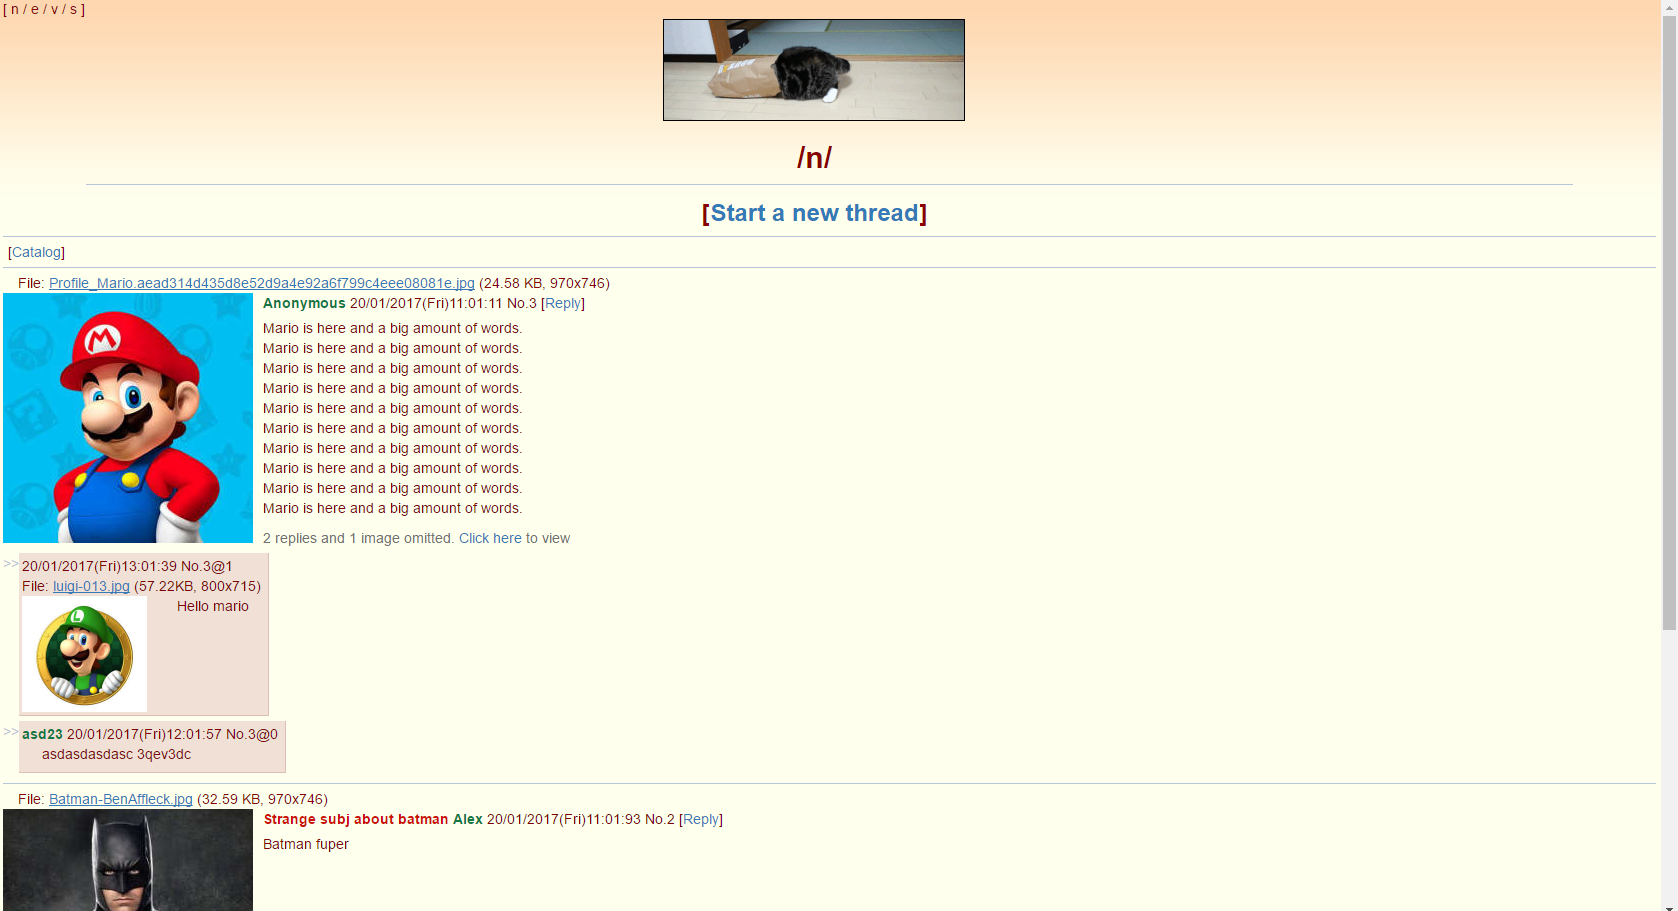
\includegraphics[width=15cm]{board-page}\\
		\caption{Board Page}
		\label{board-page}
	\end{figure}
	
	
	\begin{figure}[h]
		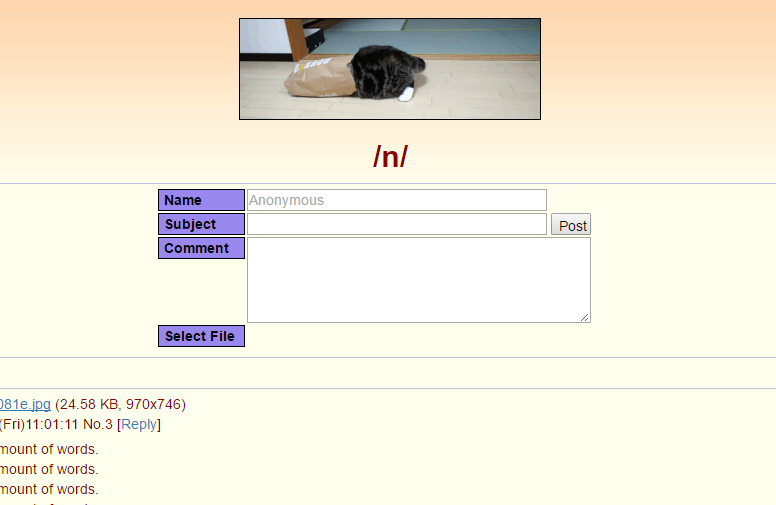
\includegraphics[width=15cm]{new-thread}\\
		\caption{New Thread Form}
		\label{new-thread}
	\end{figure}
	
	
	\begin{figure}[h]
		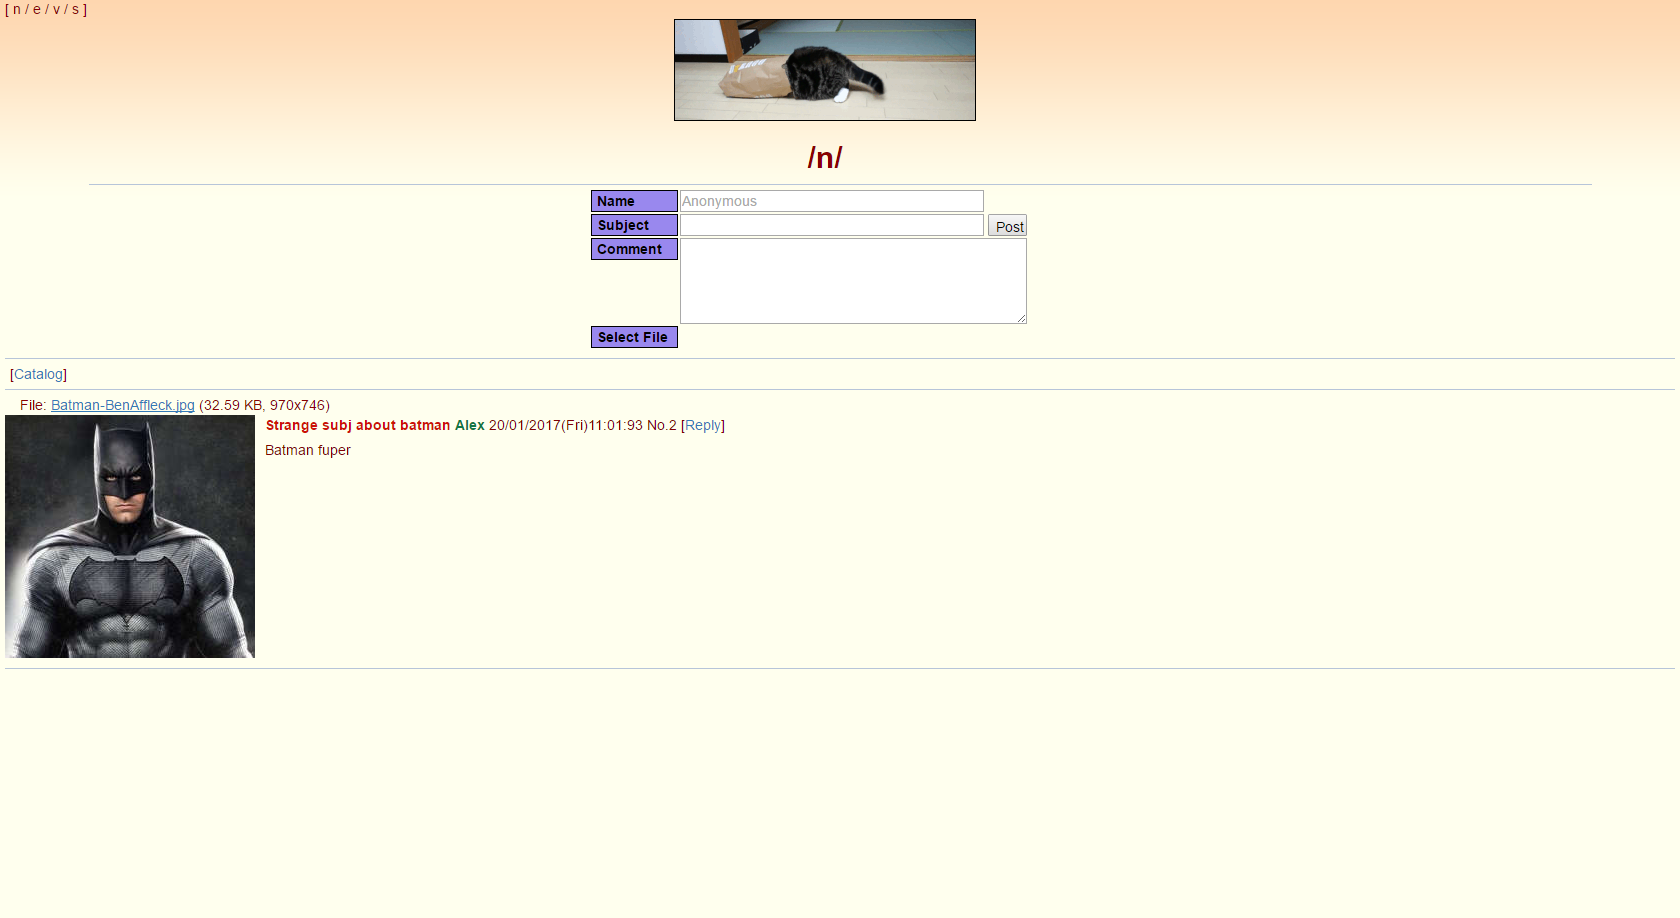
\includegraphics[width=15cm]{thread-page}\\
		\caption{Thread Page}
		\label{thread-page}
	\end{figure}
	
	
	\begin{figure}[h]
		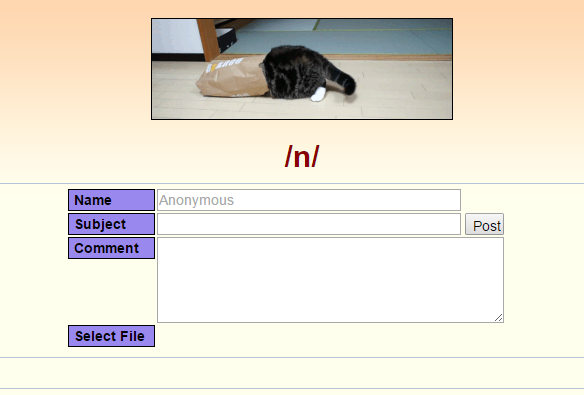
\includegraphics[width=15cm]{new-post}\\
		\caption{New post Form}
		\label{new-post}
	\end{figure}
\end{center}

\clearpage